\chapter{Management Summary}

\section{Ausgangslage}
Der Internetbrowser gehört zur Grundausstattung auf jedem Computer. Dank der grossen Verbreitung von Smartphones ist er zudem zum festen Bestandteil unseres Alltags geworden. Neue Möglichkeiten und drastische Leistungssteigerungen ermöglichen zudem die Ausführung immer komplexerer Applikationen direkt innerhalb des Browsers. So wäre der Google Mail Client oder auch Facebook, um nur zwei prominente Beispiele zu nennen, in ihrer aktuellen, interaktiven Form ohne die grossen Fortschritte im Bereich Browsertechnologie der letzten Jahre nicht umsetzbar.

Bekannte Client-Server Architekturkonzepte können da logischerweise nicht mehr zu jedem Problem passende Lösungen bereithalten. Basierend auf einem Katalog mit modernen Ansätzen soll diese Bachelorarbeit Trends im Bereich der Webapplikationen untersuchen.

Die Ergebnisse sollen dem Unterrichtsmodul ``Internettechnologien'' als Grundlage für die Konzipierung neuer Inhalte dienen.


\section{Vorgehen}

Während einer Vorstudie zu Beginn dieser Arbeit mussten drei Fragen geklärt werden:

\begin{itemize}
	\item Welche der insgesamt 28 Softwarearchitekturkonzepte aus der Aufgabenstellung sollen bearbeitet werden?
	\item Welche Applikation kann die ausgewählten Konzepte optimal veranschaulichen?
	\item Mit welcher Technologie können die ausgewählten Konzepte am besten demonstriert werden?
\end{itemize}

Nach der ausführlichen Evaluation des Konzeptkatalogs wurden 22 Konzepte ausgewählt. Um diese bestmöglich in einer Beispielapplikation demonstrieren zu können entschied das Projektteam, eine vergleichsweise einfache Aufgabenverwaltung für Studentenwohngemeinschaften zu entwickeln. Die Produktidee ``Roomies'' bietet widmet sich somit einem Thema, mit welchem sich Teilnehmer des Unterrichtmoduls ``Internettechnologien'' identifizieren und dafür begeistern können.

Um nicht nur im Bereich der Architekturkonzepte richtungsweisende Prinzipien zu untersuchen, fiel als weiterer Schritt Richtung ``Bleeding Edge'' die Technologiewahl auf einen unverbrauchten Kandidaten: Sowohl client- als auch serverseitig wird JavaScript eingesetzt.


\section{Ergebnisse}

Das Endprodukt dieser Bachelorarbeit lässt sich in drei Teile trennen.

Eine umfassende Studie analysiert alle 22 Softwarearchitekturkonzepte. Dabei wird jedes Konzept erläutert und anschliessend beschrieben, wie es in der Beispielapplikation demonstriert wurde. Als Abschluss wird jeweils eine kritische Diskussion geführt, in der das Projektteam Stellung zum Konzept nimmt.

\begin{figure}[H]
	\centering
	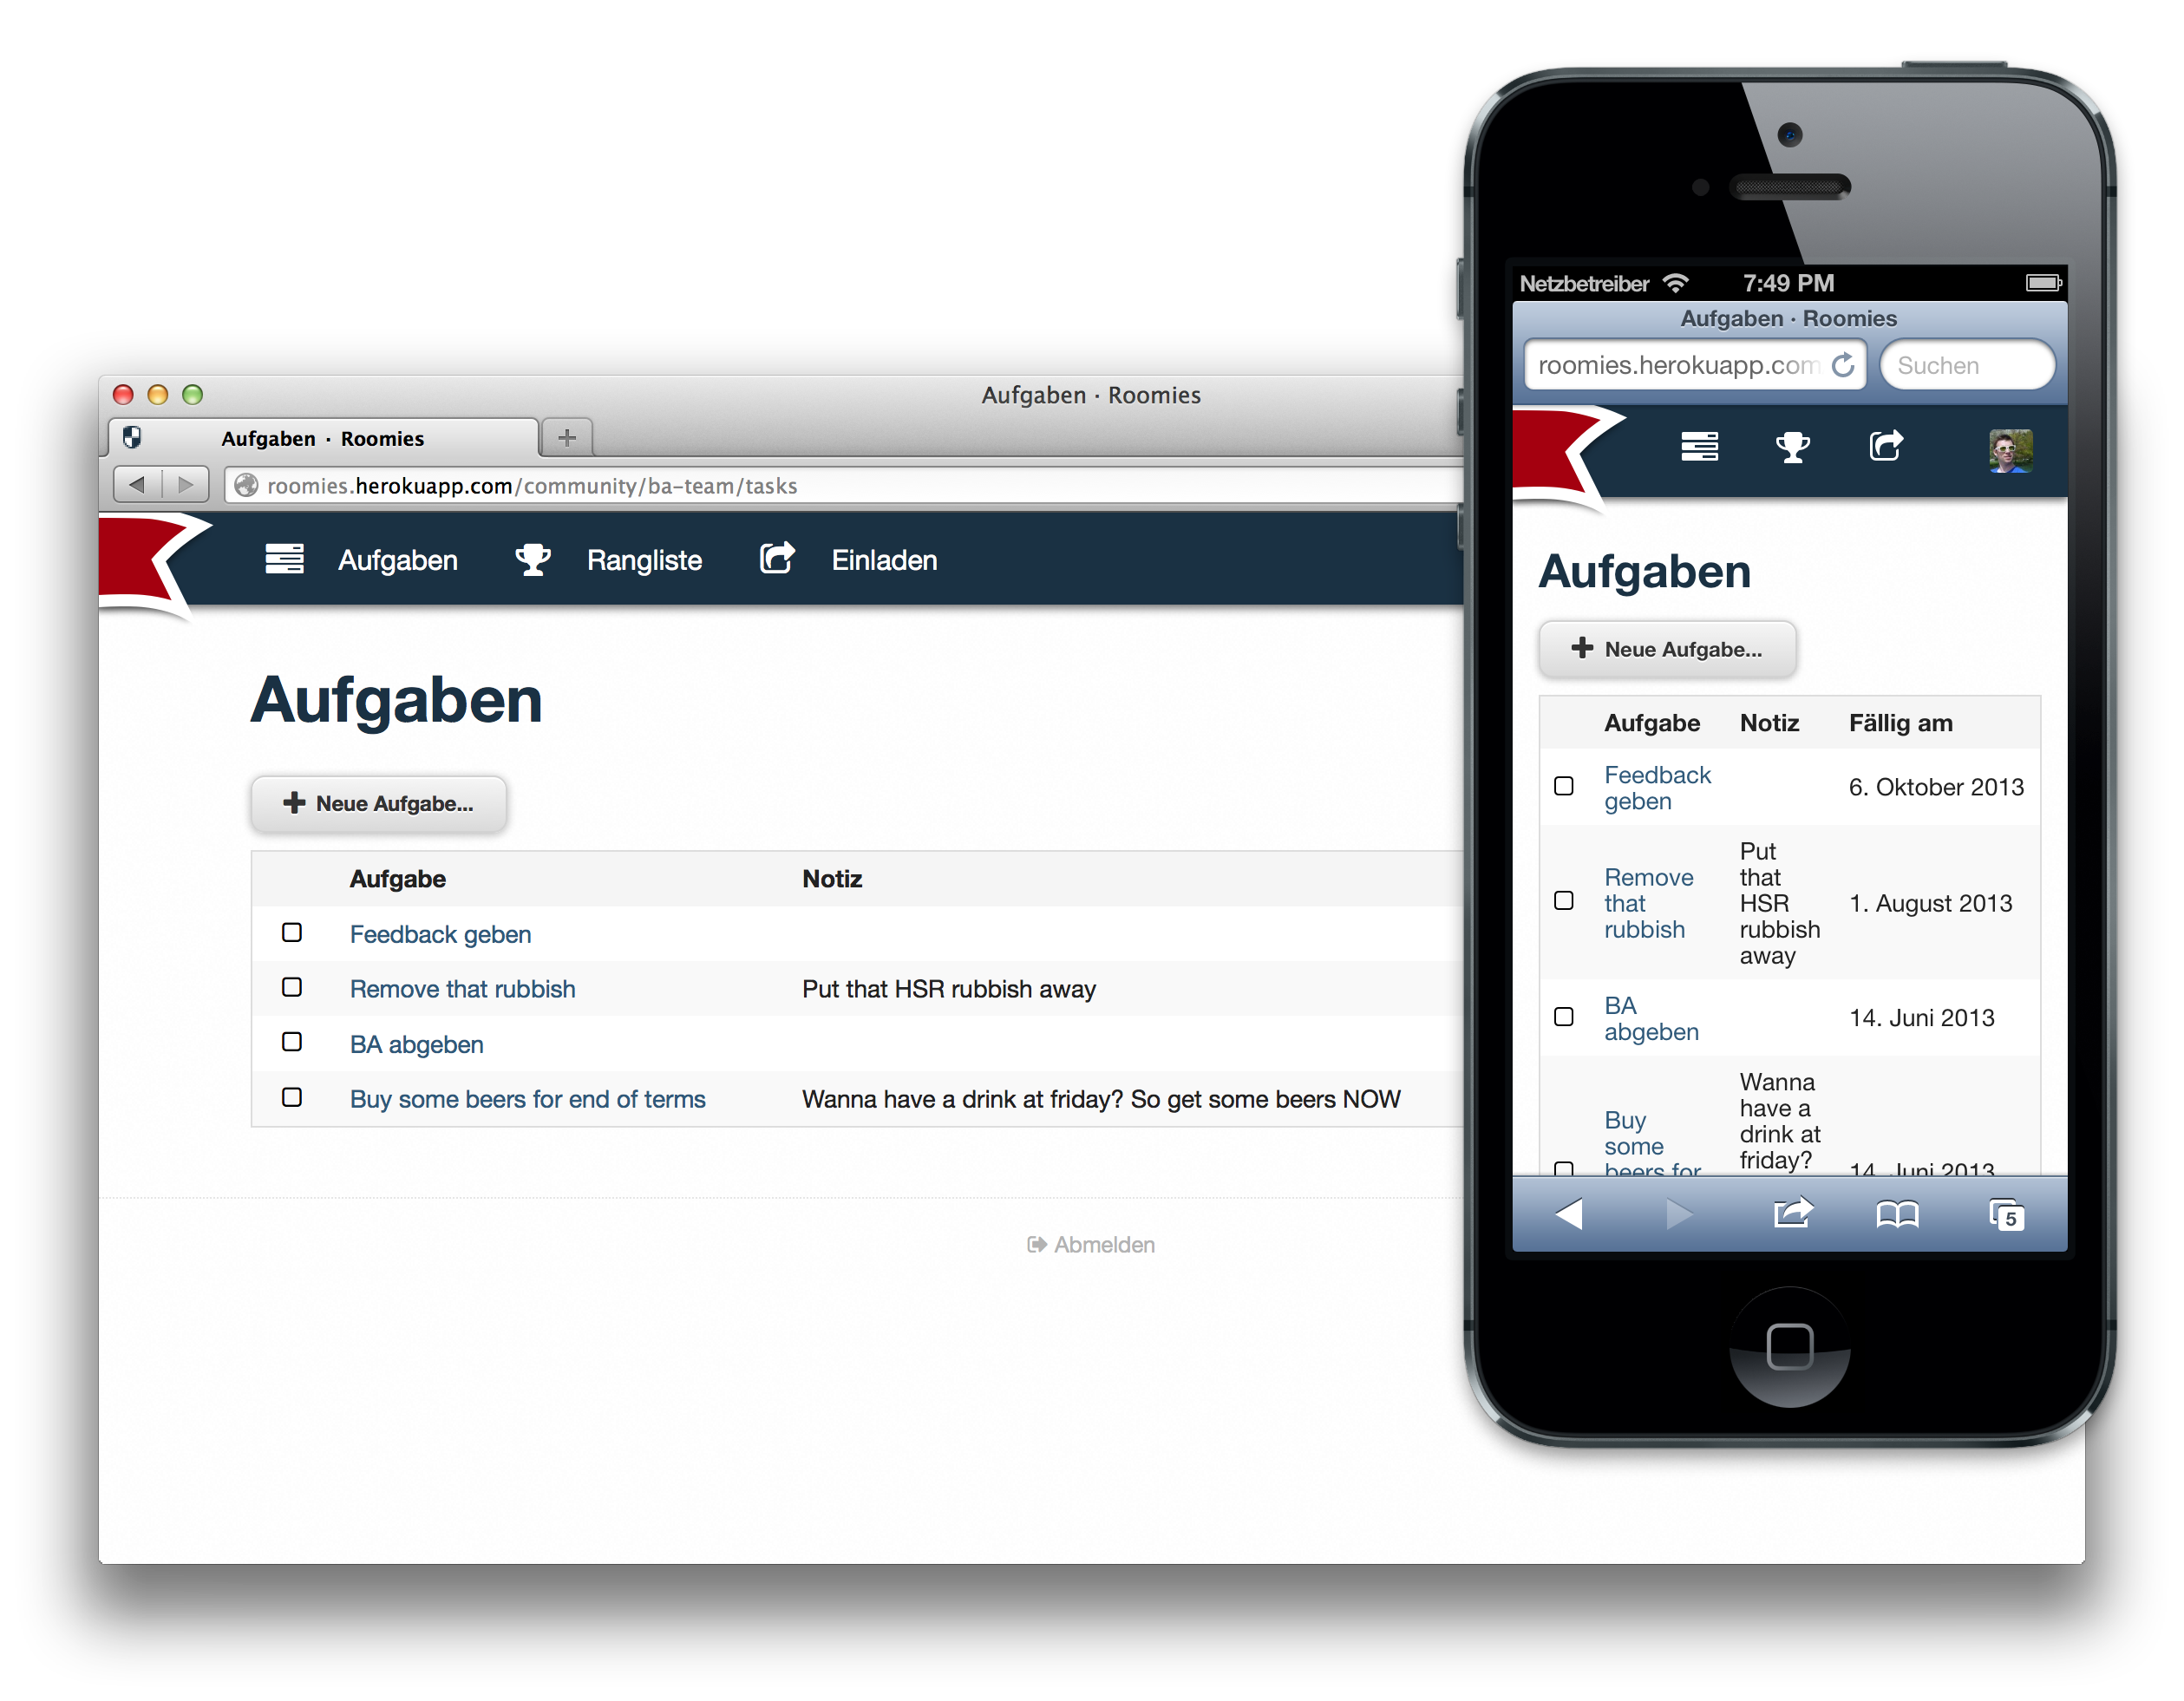
\includegraphics[width=12cm]{content/principle-demonstration/images/responsive-screenshots.png}
	\caption{Aufgabenverwaltung \emph{Roomies} zur Konzeptdemonstration}
\end{figure}

Anschauliche Quelltextbeispiele zur Studie liefert die Beispielapplikation ``Roomies''. Klar strukturierte Programmlogik ermöglicht den einfachen Zugang  zu komplexen Konzepten.

In die Umsetzung des Architekturkonzepts \emph{Unobtrusive JavaScript} wurde besonders viel Arbeit investiert. Als Belohnung ist das Framework ``barefoot'' entstanden, welches die Wiederverwendung derselben Codebasis sowohl auf dem Server als auch Client ermöglicht. Dieses Framework ist somit das dritte Produkt, welches aus dieser Arbeit hervorgeht. Es ist öffentlich zur Verwendung und Weiterentwicklung verfügbar.


\section{Ausblick}

Die vorliegenden Studie in Kombination mit der Beispielapplikation ``Roomies'' bietet eine umfassende Grundlage um Inhalte für das Unterrichtsmodul ``Internettechnologien'' neu zu konzipieren. Zwar hat das Projektteam auf die effektive Umsetzung keinen Einfluss, ist sich aber sicher, mit dieser Arbeit einen wichtigen Beitrag dazu geleistet zu haben.

``Barefoot'' ist als Framework losgelöst von dieser Bachelorarbeit wiederverwendbar. Das Projektteam ist vom Nutzen dessen überzeugt und wird sich in der Zukunft um die Weiterentwicklung und den Unterhalt von ``barefoot'' kümmern.